% Companion methods: docs/feature_similarity/README.md. No sample count in artwork.
\begin{figure*}[t]
  \centering
  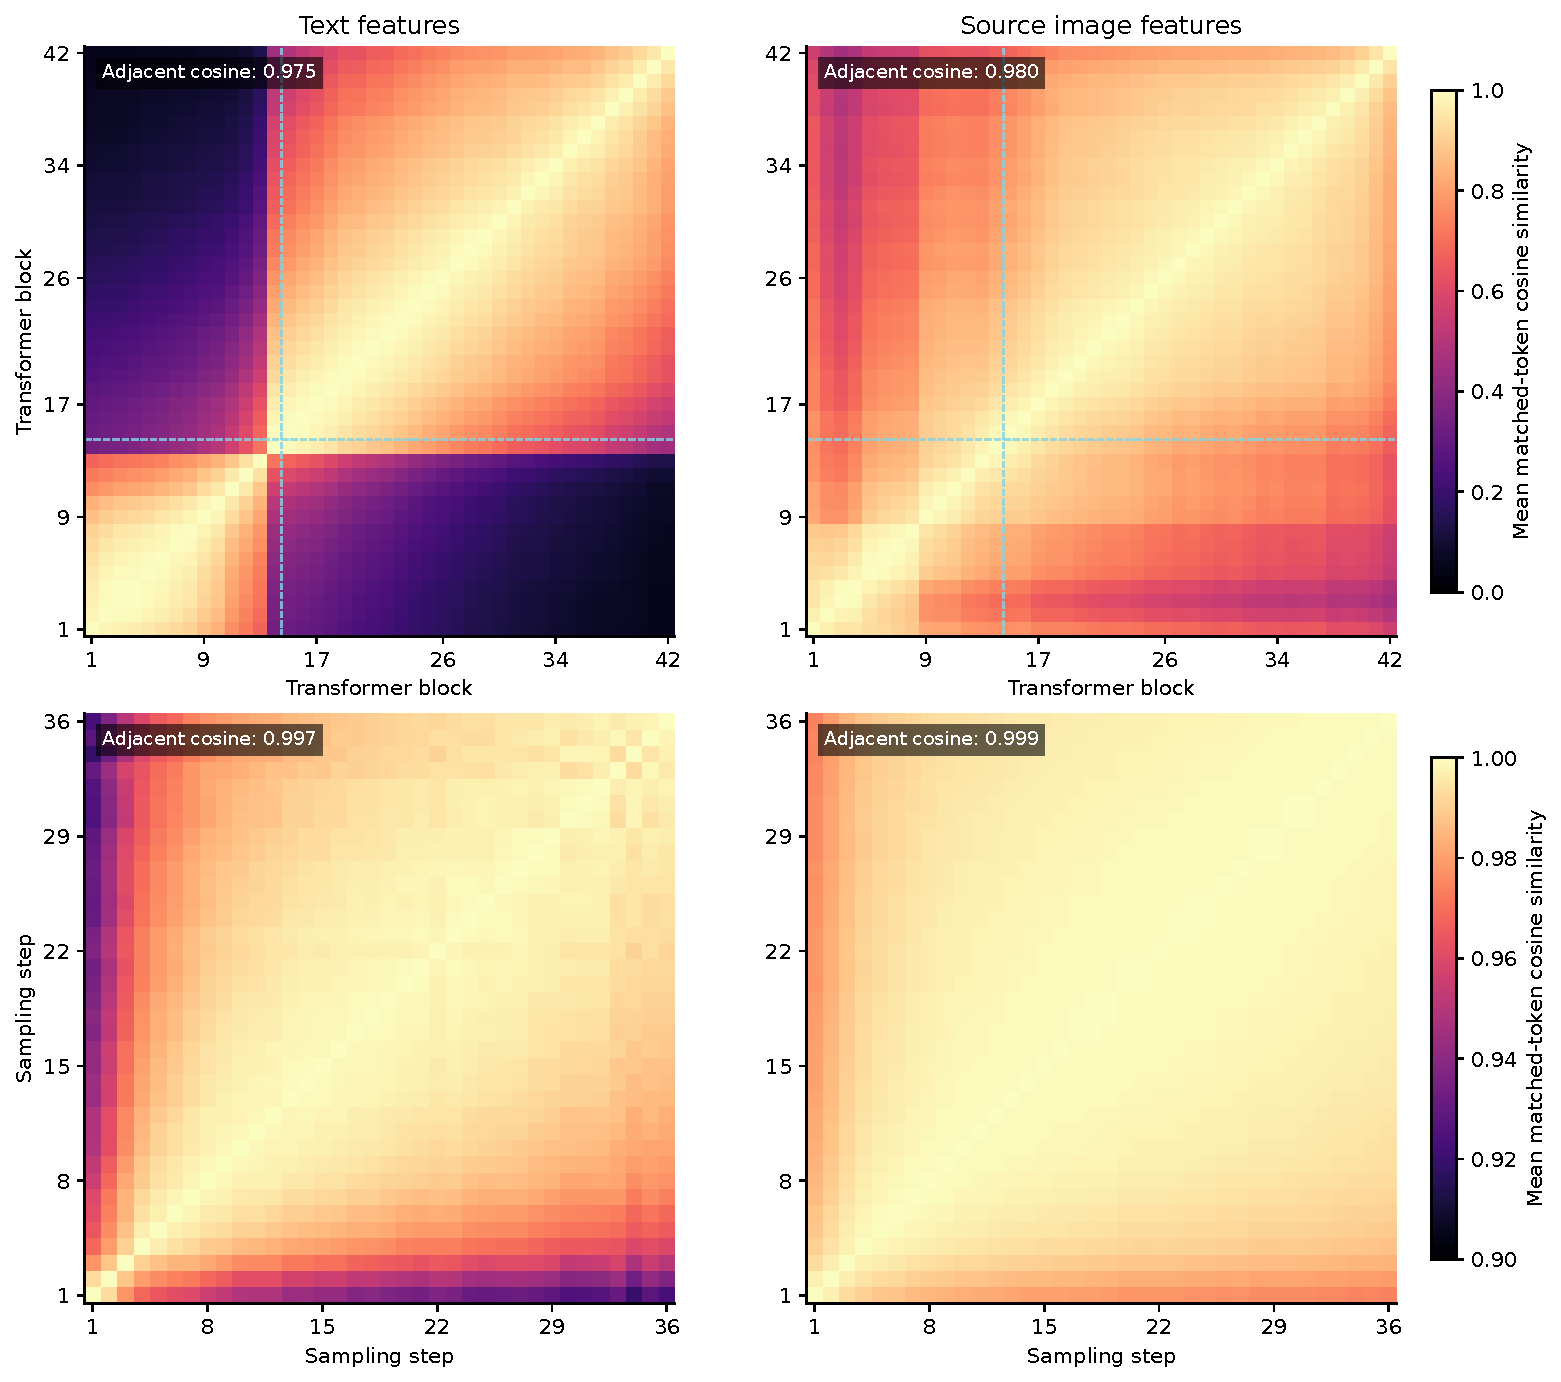
\includegraphics[width=0.83\textwidth]{docs/feature_similarity/vanilla_condition_similarity.pdf}
  \caption{Cosine similarity of conditional features in vanilla EditMGT. The upper row compares aligned instruction-token and source-image-token features across Transformer blocks; the lower row compares the same features across sampling steps. Features are taken from the positive instruction branch after each block. Colors show the mean tokenwise cosine similarity across images; dashed lines separate two-stream and single-stream blocks. Adjacent features are highly similar, whereas instruction features exhibit larger changes between distant blocks.}
  \label{fig:vanilla-condition-similarity}
\end{figure*}
